\section{Niveaumængder}
Niveaumængder tager udgangs punkt i samme logik som beviset for Sætning \ref{stn:eksistens}, og giver en metode til at finde en retningsvektor, som vil reducere objektfunktionen.
%En Niveaumængde er mængden af alle de vektorer i løsningsmængden, der har samme funktionsværdi $z$ for objektfunktionen.
\begin{defn}[Niveaumængden]
Lad $f(\vec{x})= \vec{c}^T\vec{x}$ være en objektfunktion, da kaldes
\begin{align*}
N_z = \{\vec{x}| f(\vec{x}) = z, z \in \mathds{R}\}
\end{align*}
for \textbf{niveaumængden}.
\end{defn}
Det betyder at, hvis der er tale om et lineært programmerings problem med to variable, vil niveaumængden beskrive en kurve, også kendt som en niveaukurve, mens med tre variable er der tale om et plan. 
Helt generelt beskriver niveaumængden et hyperplan.
\begin{defn}[Hyperplan]
Lad $ \vec{a} \in \mathds{R}^n$, $\vec{a}\neq \vec{0}$ og $b$ være en skalar, da kaldes en mængde for et \textbf{Hyperplan} hvis $\{ \vec{x} \in \mathds{R}^n | \vec{a}^{T}\vec{x} = \vec{b}\}$.
\end{defn}
Det ses, at hyperplanet har følgende egenskab.
\begin{stn}
Lad $N_z$ betegne niveaumængden, da er $\vec{c}$ ortogonal med hyperplanet beskrevet af $N_z$.
\end{stn}
Bemærk, at $\vec{c}$ ikke er ortogonal med $\vec{x}\in N_Z$ men med hyperplanet bestående af de punkter som $N_z$ repræsenterer.
\begin{proof}
Lad $\vec{x}, \vec{y} \in N_z$ da er hyperplanet beskrevet af $N_z$ parallel med $\vec{x}-\vec{y}$.
Tages prikproduktet af $\vec{x}-\vec{y}$ og $\vec{c}$, fåes at
\begin{align*}
\vec{c}^T(\vec{x}-\vec{y}) = \vec{c}^T\vec{x} -\vec{c}^T\vec{y} = z - z = 0,
\end{align*}
hvorfor $\vec{c}$ og $\vec{x}-\vec{y}$ er ortogonale i følge Lemma \ref{lma:vinkelret}, og dermed må $\vec{c}$ også være orthogonal med hyperplanet beskrevet af $N_z$.
\end{proof}
Den optimale værdi findes så ved at finde det mindste $z$ for hvilket niveau-hyperplanet har en ikke-tom skæring med den mulige mængde. 
Hvilket gøres ved at flytte hyperplanet så langt i den modsatte retningen af $\vec{c}$ som muligt.
\begin{stn}
Lad $f(\vec{x})=\vec{c}^T\vec{x}$ betegne objektfunktionen til et standard minimerings problem med løsningsmængde $P$, da er den 
optimale værdi givet ved
\begin{align*}
z^* = \underset{k}{\min} \, k \cdot \Vert \vec{c} \Vert ^2
\end{align*}
\label{stn:niveau}
\end{stn}
\begin{proof}
Da $N_z$ er et ægte underrum til $\mathds{R_n}$ følger det af Sætning \ref{stn:Rnorto}, at $\vec{x}$ kan omskrives til summen af en vektor parallel med $\vec{c}$, kaldet $\vec{x}_p$, og en vektor der er orthogonal med $\vec{c}$, kaldet $\vec{x}_o$. 
Dermed kan objektfunktionen omskrives til
\begin{align*}
	f(\vec{x}) & \ = \ \vec{c}^T\vec{x}\\
	f(\vec{x_p}+\vec{x_o}) & \ = \ 
	\vec{c}^T\vec{x_p}+\vec{c}^T\vec{x_o} \ = \ 
	\vec{c}^T\vec{x_p} \ = \ 
	k\cdot \vec{c}^T\vec{c} \ = \ 
	k \cdot \Vert \vec{c} \Vert ^2.
\end{align*}
Derfor kan det konkluderes, at den optimale værdi er $z* = \underset{k}{min}k \cdot \Vert \vec{c} \Vert ^2$
\end{proof}
Af Sætning \ref{stn:niveau} følger det også, at den optimale værdi er den vinkelrette afstand fra origo og  hyperplanet beskrevet  af niveaumængden, da den optimale værdi er givet, som et multiplum af længden af $\vec{c}$, der står vinkelret på hyperplanet beskrevet  af niveaumængden.
Dette kan ses i  for et maksimerings problem i Eksempel \ref{eks:maksprob3}.
\begin{eks}[Optimal løsning fundet grafisk]
Niveaukurverne $46=\vec{c}^T \vec{x}$ og $25=\vec{c}^T \vec{x}$ er på Figur \ref{fig:maksprob3} indtegnet for programmeringsprogblemet fra Eksempel \ref{eks:maksprob2}.

	\begin{center}	
		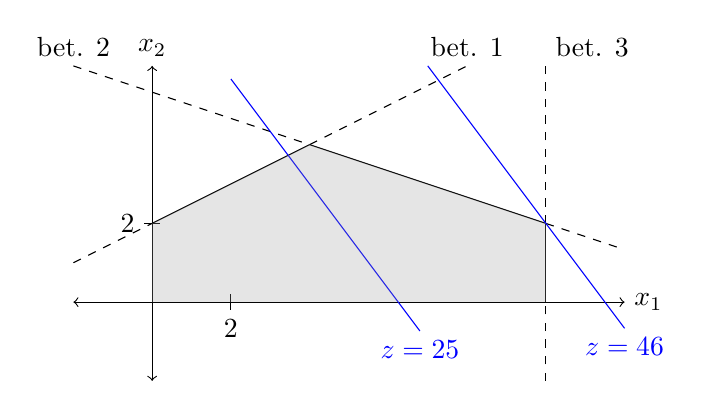
\begin{tikzpicture}
  %laver Grid. godt til når koordinater skal redigeres
  	%\draw[thin,gray!40] (-3,-1) grid (6,3); 
  %x-aksen
  	\draw[<->] (-1,0)--(6,0) node[right]{$x_1$}; 
  %y-aksen
  	\draw[<->] (0,-1)--(0,3) node[above]{$x_2$};
  	
  %akse-markeringer
  	%\node[left] (xakse) at (0,1) {2};
  	\draw[] (-0.1,1) -- (0.1,1) node[pos=0,left] {2};
  	\draw[] (1,-0.1) -- (1,0.1) node[pos=0,below] {2};
  	
  %ligning 1
	\draw[domain=-1:0,variable=\x,dashed] 	plot({\x},{0.5*\x+1});
	\draw[domain=0:2,variable=\x] 			plot({\x},{0.5*\x+1});
	\draw[domain=2:4,variable=\x,dashed] 	plot({\x},{0.5*\x+1}) node[above] {bet. 1};
	
  %ligning 2
  	\draw[domain=-1:2,variable=\x,dashed] 	plot({\x},{-(1/3)*\x+8/3}) node[above] at (-1,3) {bet. 2} ;
	\draw[domain=2:5,variable=\x] 			plot({\x},{-(1/3)*\x+8/3});
	\draw[domain=5:6,variable=\x,dashed] 	plot({\x},{-(1/3)*\x+8/3});
	

  %ligning 3
  	\draw[domain=-1:0,variable=\y,dashed] 	plot({5},{\y});
	\draw[domain=0:1,variable=\y] 			plot({5},{\y});
	\draw[domain=1:3,variable=\y,dashed] 	plot({5},{\y}) node[above right] {bet. 3};
	
  %niveaukurver
  	\draw[domain=3.5:6,variable=\x,blue] plot({\x},{-(4/3)*\x+23/3}) node[below] {$z=46$};
  	\draw[domain=1:3.4,variable=\x,blue] plot({\x},{-(4/3)*\x+25/6}) node[below] {$z=25$};
  	
  %c-vektor
  	%\draw[->,thick,red] (0,0) -- (2,1.5);

  %løsningsmængden skraveret
	\fill[gray!80,nearly transparent] (0,0) -- (0,1) -- (2,2) -- (5,1) --(5,0) --  cycle;
\end{tikzpicture}
		\captionof{figure}{Optimal løsning i den mulige mængde fundet som skæring med ligningen $z=46$.}
		\label{fig:maksprob3}
	\end{center}
	
På figuren ses det, at den største funktionsværdi $z=46$ findes i skæringen mellem bibetingelse 2 og 3.
Ved at løse bibetingelse 2 og 3 som 2 ligninger med 2 ubekendte findes det at den optimale løsning er $\vec{x}=\rvect{10 & 2}^T.$
\label{eks:maksprob3}
\end{eks}
%%%%%%%%%%%%%%%%%%%%%%%%%%%%%%%%%%%%%%%%%%%%%%%%%%%%%%%%%%%%%%%%%%%%%%%%%%%%%%%%%%%%%%
%%%%%%%%%%%%%%%%%%%%%%%%%%%%%%%%%%%%%%%%%%%%%%%%%%%%%%%%%%%%%%%%%%%%%%%%%%%%%%%%%%%%%%
%\texttt{
%\subsection{Niveaukurver}
%Niveaukurver dannes ved fastsættelsen af en funktionsværdi $z=\vec{c}^T \vec{x}$. Niveaukurven er derved mængden af alle vektorer $\vec{x}$, som løser ligningen. Da målet er at maksimere $z$, er målet at finde den største $z$ for hvilken niveaukurven har en ikke-tom skæring med den mulige mængde. 
%
%En løsningsvektor $\vec{x}$ kan omskrives til summen af en vektor parallel med $\vec{c}$, kaldet $\vec{x}_p$, og en vektor orthogonal med $\vec{c}$, kaldet $\vec{x}_o$. Her gælder det derved at, $\vec{x}_p=k\cdot \vec{c}$ for en skalar $k$, og at $\vec{x}_o^T \vec{c}=0$. Dette er muligt, da vektorrummet der er orthogonalt med $\vec{c}$ har dimension $n-1$, mens rummet dannet af $\vec{c}$ har dimension $1$. Da vil vektorrummet dannet af summen af disse rum have dimension $n$, da de to rum er orthononale. Derved kan alle løsningsvektorer $\vec{x}$ udtrykkes som summen af en vektor fra hvert af de to rum.
%
%\begin{align*}
%	f(\vec{x}) & \ = \ \vec{c}^T\vec{x}\\
%	f(\vec{x_p}+\vec{x_o}) & \ = \ 
%	\vec{c}^T\vec{x_p}+\vec{c}^T\vec{x_o} \ = \ 
%	\vec{c}^T\vec{x_p} \ = \ 
%	k\cdot \vec{c}^T\vec{c} \ = \ 
%	k \cdot \Vert \vec{c} \Vert ^2
%\end{align*}
%Da funktionsværdien derved er lig $k \cdot \Vert \vec{c} \Vert ^2$ gælder det derved om at maksimere $k$ for maksimeringsproblemer og at minimere $k$ for minimeringsproblemer. 
%
%
%Dette kan ses i Eksempel \ref{eks:maksprob3}.
%\begin{comment}
%Bør niveaukurve defineres????? Hvordan kan dette bruges, for at finde $z$ er egentlig bare en omskrivning, så der mangler noget argumentation for at $z$ bliver større jo længere væk fra origo man er, hvilket giver ret god mening, men er svært at argumentere for uden at starte på geometri, så måske hele dette afsnit skulle flyttes, måske skal alt om løsninger skal flyttes til geometri?
%\end{comment}
%
%
%\begin{eks}[Optimal løsning fundet grafisk]
%Niveaukurverne $46=\vec{c}^T \vec{x}$ og $25=\vec{c}^T \vec{x}$ er på Figur \ref{fig:maksprob3} indtegnet for programmeringsprogblemet fra Eksempel \ref{eks:maksprob2}.
%
%	\begin{center}	
%		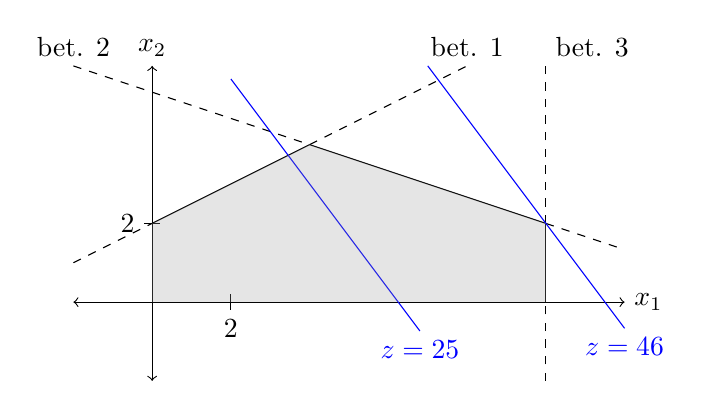
\begin{tikzpicture}
  %laver Grid. godt til når koordinater skal redigeres
  	%\draw[thin,gray!40] (-3,-1) grid (6,3); 
  %x-aksen
  	\draw[<->] (-1,0)--(6,0) node[right]{$x_1$}; 
  %y-aksen
  	\draw[<->] (0,-1)--(0,3) node[above]{$x_2$};
  	
  %akse-markeringer
  	%\node[left] (xakse) at (0,1) {2};
  	\draw[] (-0.1,1) -- (0.1,1) node[pos=0,left] {2};
  	\draw[] (1,-0.1) -- (1,0.1) node[pos=0,below] {2};
  	
  %ligning 1
	\draw[domain=-1:0,variable=\x,dashed] 	plot({\x},{0.5*\x+1});
	\draw[domain=0:2,variable=\x] 			plot({\x},{0.5*\x+1});
	\draw[domain=2:4,variable=\x,dashed] 	plot({\x},{0.5*\x+1}) node[above] {bet. 1};
	
  %ligning 2
  	\draw[domain=-1:2,variable=\x,dashed] 	plot({\x},{-(1/3)*\x+8/3}) node[above] at (-1,3) {bet. 2} ;
	\draw[domain=2:5,variable=\x] 			plot({\x},{-(1/3)*\x+8/3});
	\draw[domain=5:6,variable=\x,dashed] 	plot({\x},{-(1/3)*\x+8/3});
	

  %ligning 3
  	\draw[domain=-1:0,variable=\y,dashed] 	plot({5},{\y});
	\draw[domain=0:1,variable=\y] 			plot({5},{\y});
	\draw[domain=1:3,variable=\y,dashed] 	plot({5},{\y}) node[above right] {bet. 3};
	
  %niveaukurver
  	\draw[domain=3.5:6,variable=\x,blue] plot({\x},{-(4/3)*\x+23/3}) node[below] {$z=46$};
  	\draw[domain=1:3.4,variable=\x,blue] plot({\x},{-(4/3)*\x+25/6}) node[below] {$z=25$};
  	
  %c-vektor
  	%\draw[->,thick,red] (0,0) -- (2,1.5);

  %løsningsmængden skraveret
	\fill[gray!80,nearly transparent] (0,0) -- (0,1) -- (2,2) -- (5,1) --(5,0) --  cycle;
\end{tikzpicture}
%		\captionof{figure}{Optimal løsning i den mulige mængde fundet som skæring med ligningen $z=46$.}
%		\label{fig:maksprob3}
%	\end{center}
%	
%På figuren ses det, at den største funktionsværdi $z=46$ findes i skæringen mellem bibetingelse 2 og 3.
%Ved at løse bibetingelse 2 og 3 som 2 ligninger med 2 ubekendte findes det at den optimale løsning er $\vec{x}=\rvect{10 & 2}^T.$
%\label{eks:maksprob3}
%\end{eks}}